% Options for packages loaded elsewhere
\PassOptionsToPackage{unicode}{hyperref}
\PassOptionsToPackage{hyphens}{url}
\documentclass[
]{article}
\usepackage{xcolor}
\usepackage{amsmath,amssymb}
\setcounter{secnumdepth}{-\maxdimen} % remove section numbering
\usepackage{iftex}
\ifPDFTeX
  \usepackage[T1]{fontenc}
  \usepackage[utf8]{inputenc}
  \usepackage{textcomp} % provide euro and other symbols
\else % if luatex or xetex
  \usepackage{unicode-math} % this also loads fontspec
  \defaultfontfeatures{Scale=MatchLowercase}
  \defaultfontfeatures[\rmfamily]{Ligatures=TeX,Scale=1}
\fi
\usepackage{lmodern}
\ifPDFTeX\else
  % xetex/luatex font selection
\fi
% Use upquote if available, for straight quotes in verbatim environments
\IfFileExists{upquote.sty}{\usepackage{upquote}}{}
\IfFileExists{microtype.sty}{% use microtype if available
  \usepackage[]{microtype}
  \UseMicrotypeSet[protrusion]{basicmath} % disable protrusion for tt fonts
}{}
\makeatletter
\@ifundefined{KOMAClassName}{% if non-KOMA class
  \IfFileExists{parskip.sty}{%
    \usepackage{parskip}
  }{% else
    \setlength{\parindent}{0pt}
    \setlength{\parskip}{6pt plus 2pt minus 1pt}}
}{% if KOMA class
  \KOMAoptions{parskip=half}}
\makeatother
\usepackage{graphicx}
\makeatletter
\newsavebox\pandoc@box
\newcommand*\pandocbounded[1]{% scales image to fit in text height/width
  \sbox\pandoc@box{#1}%
  \Gscale@div\@tempa{\textheight}{\dimexpr\ht\pandoc@box+\dp\pandoc@box\relax}%
  \Gscale@div\@tempb{\linewidth}{\wd\pandoc@box}%
  \ifdim\@tempb\p@<\@tempa\p@\let\@tempa\@tempb\fi% select the smaller of both
  \ifdim\@tempa\p@<\p@\scalebox{\@tempa}{\usebox\pandoc@box}%
  \else\usebox{\pandoc@box}%
  \fi%
}
% Set default figure placement to htbp
\def\fps@figure{htbp}
\makeatother
\setlength{\emergencystretch}{3em} % prevent overfull lines
\providecommand{\tightlist}{%
  \setlength{\itemsep}{0pt}\setlength{\parskip}{0pt}}
\usepackage{bookmark}
\IfFileExists{xurl.sty}{\usepackage{xurl}}{} % add URL line breaks if available
\urlstyle{same}
\hypersetup{
  hidelinks,
  pdfcreator={LaTeX via pandoc}}

\author{}
\date{}

\begin{document}

\section{Paper 1: Dual Geometry of Wavelength Space and Frequency
Space}\label{paper-1-dual-geometry-of-wavelength-space-and-frequency-space}

\subsection{A Geometric and Topological Observational Model of
Reciprocal Conditions, Logarithmic Representation, and
Uncertainty-Weighted
Counting}\label{a-geometric-and-topological-observational-model-of-reciprocal-conditions-logarithmic-representation-and-uncertainty-weighted-counting}

\textbf{Author}: Noriaki Kihara\\
\textbf{Affiliation}: WF System Co., Ltd.\\
\textbf{ORCID}: 0009-0004-6753-4020\\
\textbf{Version}: v0.3\\
\textbf{Date}: June 2026\\
\textbf{DOI (this version)}: 10.5281/zenodo.20588037\\
\textbf{Concept DOI}: 10.5281/zenodo.20588036\\
\textbf{License}: CC BY 4.0

\begin{center}\rule{0.5\linewidth}{0.5pt}\end{center}

\subsection{Abstract}\label{abstract}

In this paper we place between the wavelength components \(\lambda_n\)
and the frequency components \(\nu_n\) the reciprocal duality condition

\[
\lambda_n=\frac{1}{\nu_n}
\]

and observe the structure that emerges when we further impose, on the
wavelength space and the frequency space respectively, the constant
sum-of-squares geometric conditions

\[
\sum_{n=1}^{d} \lambda_n^2=\Lambda^2,\qquad
\sum_{n=1}^{d} \nu_n^2=\mathcal{N}^2 .
\]

The purpose of this paper is not to derive physical entities such as
spacetime, mass, energy, or momentum. The quantities \(\lambda_n\) and
\(\nu_n\) here are model variables used to describe the dual geometric
structure of the wavelength space and the frequency space. Accordingly,
we do not identify \(\nu_n\) with time-frequency, energy, momentum, or
any other quantity of standard physics.

In the ordinary representation the reciprocal duality appears as the
hyperbola

\[
\lambda\nu=1 ,
\]

but under the logarithmic change of variables

\[
q_n=\log \lambda_n,\qquad p_n=\log \nu_n
\]

it is simplified to the sign-reversal symmetry

\[
p_n=-q_n .
\]

We also confirm that, whereas in one dimension the solution is fixed to
essentially a single point with almost no freedom for redistribution
among components, a 5-component / 1-constraint system retains four
degrees of freedom. Finally, when an actual 4-dimensional lattice is
chosen in the frequency space or the wavelength space, we formulate the
corresponding counting method. In particular, we define the
fully-inscribed count without uncertainty (\(\delta=0\)) and the
weighted count with uncertainty (\(\delta>0\)). However, this paper does
not derive the value of \(\delta\) or the form of the weight function.
Their determination is outside the scope of this paper and is left to
subsequent work.

\begin{center}\rule{0.5\linewidth}{0.5pt}\end{center}

\subsection{Keywords}\label{keywords}

wavelength space, frequency space, reciprocal duality, logarithmic
representation, sign-reversal symmetry, four degrees of freedom,
4-dimensional lattice, unit-cell counting, uncertainty, geometric
observational model, topological observational model

\begin{center}\rule{0.5\linewidth}{0.5pt}\end{center}

\subsection{1. Introduction}\label{introduction}

Rather than presupposing space or spacetime as a known background, it is
useful as a thought experiment to observe what geometric degrees of
freedom arise naturally from the duality between wavelength and
frequency.

In this paper we place between the wavelength components \(\lambda_n\)
and the frequency components \(\nu_n\) the simplest reciprocal duality
condition

\[
\lambda_n=\frac{1}{\nu_n} .
\]

A point to note here is that the ``wavelength'' and ``frequency'' of
this paper are not to be immediately identified with physical quantities
of standard physics. We treat \(\lambda_n\) as a scale component along
each axis and \(\nu_n\) as its reciprocal component. For convenience we
use the words ``wavelength'' and ``frequency,'' but \(\nu_n\) is not
identified with time-frequency, energy, momentum, or other physical
quantities.

The question of this paper can be stated as follows.

\begin{quote}
When the wavelength space and the frequency space are connected by a
reciprocal duality and each additionally carries a norm-preserving
condition, what kind of degrees of freedom, symmetry, and counting
structure arise naturally?
\end{quote}

This paper does not claim the derivation of 4-dimensional spacetime or
the completion of a physical theory. It is rather an observational model
of what geometric and topological structure is produced by the
reciprocal duality placed between the wavelength space and the frequency
space.

\begin{center}\rule{0.5\linewidth}{0.5pt}\end{center}

\subsection{2. Basic Setup}\label{basic-setup}

\subsubsection{2.1 Wavelength space}\label{wavelength-space}

Let the \(d\) wavelength components be

\[
\lambda=(\lambda_1,\lambda_2,\ldots,\lambda_d) .
\]

We impose the constant sum-of-squares condition on the wavelength space,

\[
\sum_{n=1}^{d} \lambda_n^2=\Lambda^2 ,
\]

where \(\Lambda\) represents a composite wavelength scale, or the norm
radius in the wavelength space.

\subsubsection{2.2 Frequency space}\label{frequency-space}

Similarly, let the \(d\) frequency components be

\[
\nu=(\nu_1,\nu_2,\ldots,\nu_d) .
\]

We impose the constant sum-of-squares condition on the frequency space,

\[
\sum_{n=1}^{d} \nu_n^2=\mathcal{N}^2 ,
\]

where \(\mathcal{N}\) represents a composite frequency scale, or the
norm radius in the frequency space.

\subsubsection{2.3 Reciprocal duality
condition}\label{reciprocal-duality-condition}

Between the wavelength components and the frequency components we place
the componentwise reciprocal duality condition

\[
\lambda_n\nu_n=1 ,
\]

that is,

\[
\lambda_n=\frac{1}{\nu_n} .
\]

By this condition the wavelength space and the frequency space are not
independent but are dual spaces connected by a reciprocal map. When one
component is large, the corresponding other component is small. Hence
this is not a symmetry of identical form but a dual symmetry that
includes inversion.

\begin{center}\rule{0.5\linewidth}{0.5pt}\end{center}

\subsection{3. The One-Dimensional Case}\label{the-one-dimensional-case}

In one dimension the conditions are

\[
\lambda^2=\Lambda^2,\qquad
\nu^2=\mathcal{N}^2,\qquad
\lambda\nu=1 .
\]

Considering only positive wavelength and positive frequency,

\[
\lambda=\Lambda,\qquad
\nu=\mathcal{N} ,
\]

and necessarily

\[
\Lambda\mathcal{N}=1 .
\]

Therefore, in one dimension the solution is fixed to

\[
\lambda=\Lambda,\qquad
\nu=\frac{1}{\Lambda} .
\]

This shows that in a one-dimensional system the degrees of freedom
essentially vanish and there is almost no room for redistribution among
components. That is, a one-dimensional system formally possesses a
solution, but has almost no margin for expressing a closed dual geometry
or an observational thickness.

\begin{center}\rule{0.5\linewidth}{0.5pt}\end{center}

\subsection{4. Multicomponent Systems and the Emergence of Four Degrees
of
Freedom}\label{multicomponent-systems-and-the-emergence-of-four-degrees-of-freedom}

Consider the 5-component case.

In the wavelength space we impose

\[
\sum_{n=1}^{5} \lambda_n^2=\Lambda^2 .
\]

In the frequency space we impose

\[
\sum_{n=1}^{5} \nu_n^2=\mathcal{N}^2 .
\]

On each component we impose

\[
\lambda_n\nu_n=1 .
\]

Here, since the five components are subject to one sum-of-squares
constraint, ideally

\[
5-1=4
\]

degrees of freedom remain.

These four degrees of freedom are an important object of observation in
this paper. However, we do not immediately identify these four degrees
of freedom with the 4-dimensionality of physical spacetime. What we
treat here is a degree of freedom that appears purely on the dual
geometry.

\subsubsection{4.1 Existence condition}\label{existence-condition}

Setting

\[
a_n=\lambda_n^2>0 ,
\]

we have

\[
\sum_{n=1}^{5} a_n=\Lambda^2 ,
\]

and, from

\[
\nu_n=\frac{1}{\lambda_n} ,
\]

it follows that

\[
\sum_{n=1}^{5} \frac{1}{a_n}=\mathcal{N}^2 .
\]

By a Cauchy--Schwarz type inequality,

\[
\left(\sum_{n=1}^{5} a_n\right)
\left(\sum_{n=1}^{5} \frac{1}{a_n}\right)\ge 25 .
\]

Therefore

\[
\Lambda^2\mathcal{N}^2\ge 25 ,
\]

that is,

\[
\Lambda\mathcal{N}\ge 5
\]

is a necessary condition.

Equality holds when all \(a_n\) are equal, namely

\[
a_1=a_2=a_3=a_4=a_5=\frac{\Lambda^2}{5} .
\]

\begin{center}\rule{0.5\linewidth}{0.5pt}\end{center}

\subsection{5. Logarithmic
Representation}\label{logarithmic-representation}

The reciprocal duality condition

\[
\lambda_n=\frac{1}{\nu_n}
\]

is expressed in the ordinary representation as a hyperbolic relation.

However, introducing the logarithmic variables

\[
q_n=\log\lambda_n,\qquad
p_n=\log\nu_n ,
\]

since

\[
\log\lambda_n=-\log\nu_n ,
\]

we obtain

\[
p_n=-q_n .
\]

That is, the reciprocal duality which in the ordinary representation is
the hyperbola

\[
\lambda\nu=1
\]

is, in logarithmic space, the straight line of slope \(-1\),

\[
p=-q .
\]

\begin{center}\rule{0.5\linewidth}{0.5pt}\end{center}

\subsection{6. Introduction of Uncertainty and Its
Scope}\label{introduction-of-uncertainty-and-its-scope}

The above conditions are clear as an ideal state but are strongly
constraining. We therefore formally introduce an uncertainty on the
observed values or lattice values.

However, this paper does not derive the value of the uncertainty width
\(\delta\). Nor do we identify \(\delta\) with any specific physical
uncertainty. What we do in this paper is to define a counting formalism
that includes \(\delta\).

As an example of placing an integer lattice with a fractional
fluctuation on the frequency side, we may write

\[
\nu_n=m_n+\epsilon_n,\qquad
m_n\in\mathbb{Z},\qquad
|\epsilon_n|\le \delta_\nu .
\]

The wavelength side is then induced from the reciprocal duality
condition as

\[
\lambda_n=\frac{1}{m_n+\epsilon_n} .
\]

Taking the ideal integer mode as

\[
\nu_n^{(0)}=m_n ,
\]

the corresponding ideal wavelength is

\[
\lambda_n^{(0)}=\frac{1}{m_n} .
\]

The wavelength including the fluctuation is

\[
\lambda_n^{\mathrm{obs}}=
\frac{1}{m_n+\epsilon_n} .
\]

Hence the wavelength-side fluctuation is

\[
\Delta\lambda_n
=
\frac{1}{m_n+\epsilon_n}
-
\frac{1}{m_n}
=
-\frac{\epsilon_n}{m_n(m_n+\epsilon_n)} .
\]

When \(|\epsilon_n|\ll m_n\), to first order

\[
\Delta\lambda_n\approx
-\frac{\epsilon_n}{m_n^2} .
\]

This formula shows that a fractional fluctuation on the frequency side
appears on the wavelength side as a fluctuation of the opposite sign.
However, the values and distributions of \(\epsilon_n\) and
\(\delta_\nu\) are not determined in this paper.

\begin{center}\rule{0.5\linewidth}{0.5pt}\end{center}

\subsection{7. Explanation by Figures}\label{explanation-by-figures}

\subsubsection{\texorpdfstring{Figure 1: Schematic of the
\(\lambda\)--\(\nu\) dual
constraint}{Figure 1: Schematic of the \textbackslash lambda--\textbackslash nu dual constraint}}\label{figure-1-schematic-of-the-lambdanu-dual-constraint}

\begin{figure}
\centering
\pandocbounded{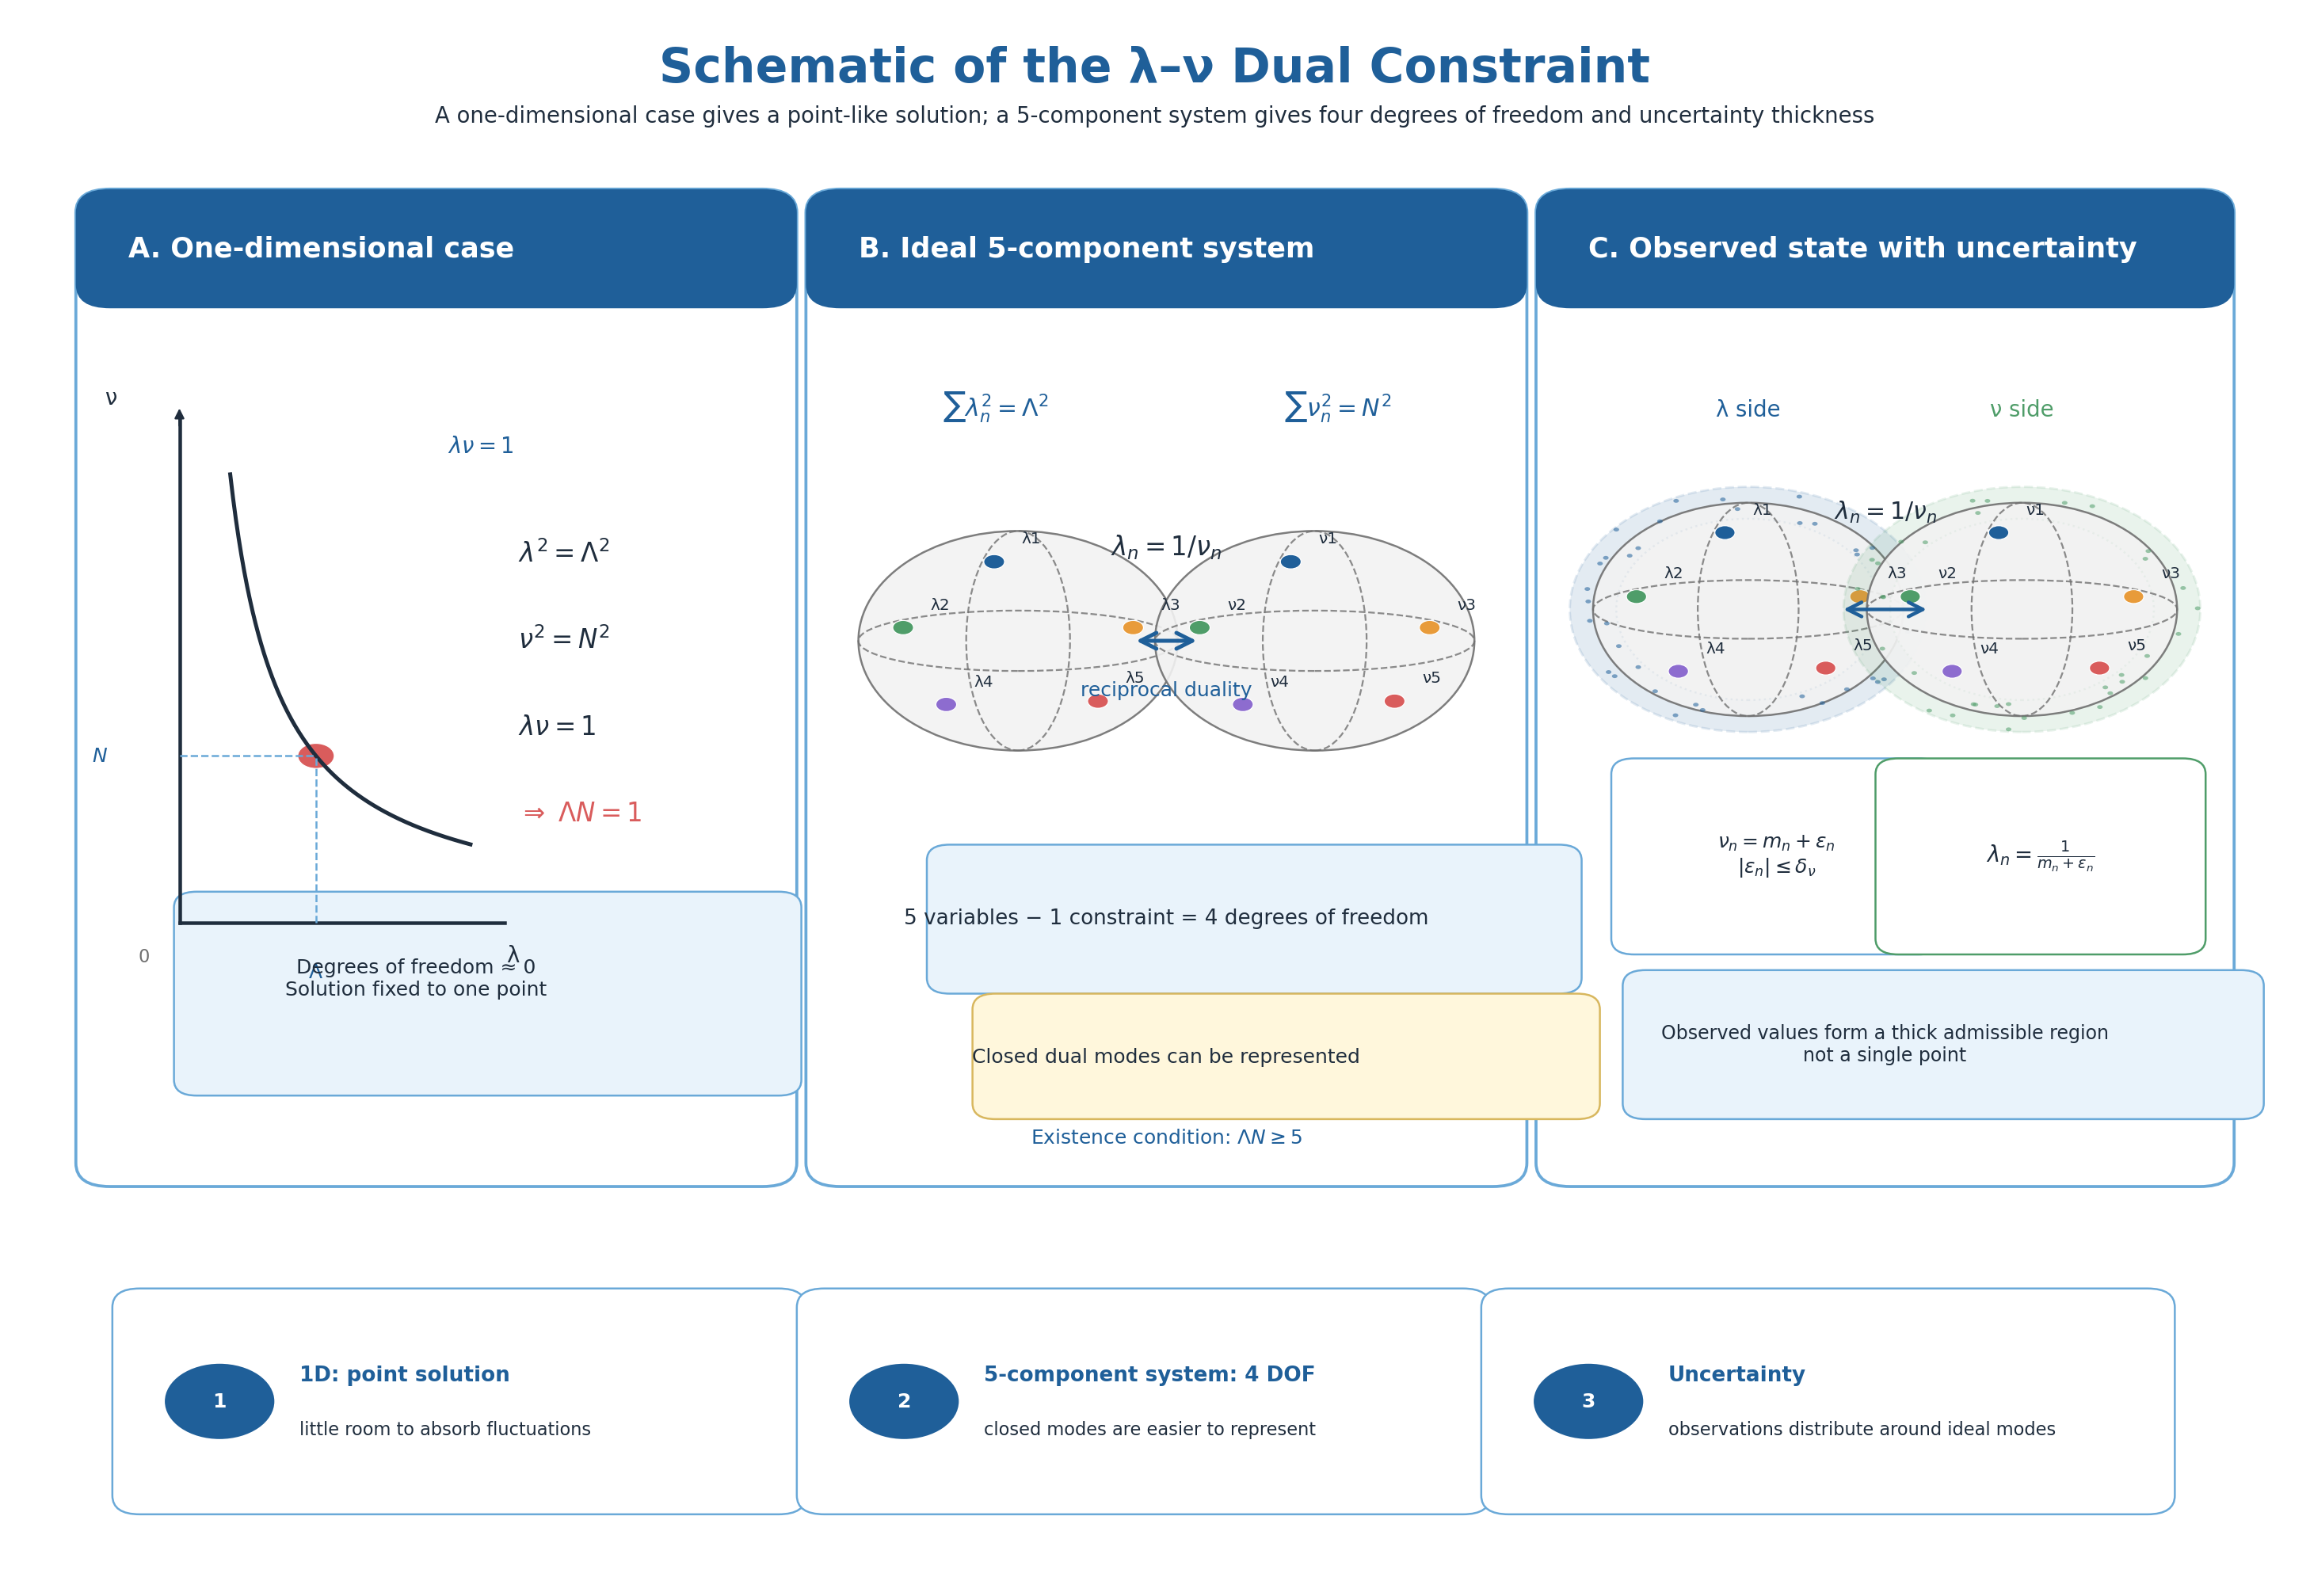
\includegraphics[keepaspectratio,alt={Schematic of the \textbackslash lambda--\textbackslash nu dual constraint}]{./figure1_lambda_nu_dual_constraint_EN.png}}
\caption{Schematic of the \(\lambda\)--\(\nu\) dual constraint}
\end{figure}

\textbf{Figure 1.} In one dimension, the conditions
\(\lambda^2=\Lambda^2\), \(\nu^2=\mathcal{N}^2\), \(\lambda\nu=1\) fix
the solution to essentially a single point. In contrast, a 5-component /
1-constraint system retains four degrees of freedom, leaving room to
build a dual geometry. Introducing uncertainty, the situation can be
represented as an observational region having thickness around the ideal
constraint. However, the magnitude of that thickness is not derived in
this paper.

\subsubsection{\texorpdfstring{Figure 2: Logarithmic representation of
the \(\lambda\)--\(\nu\)
duality}{Figure 2: Logarithmic representation of the \textbackslash lambda--\textbackslash nu duality}}\label{figure-2-logarithmic-representation-of-the-lambdanu-duality}

\begin{figure}
\centering
\pandocbounded{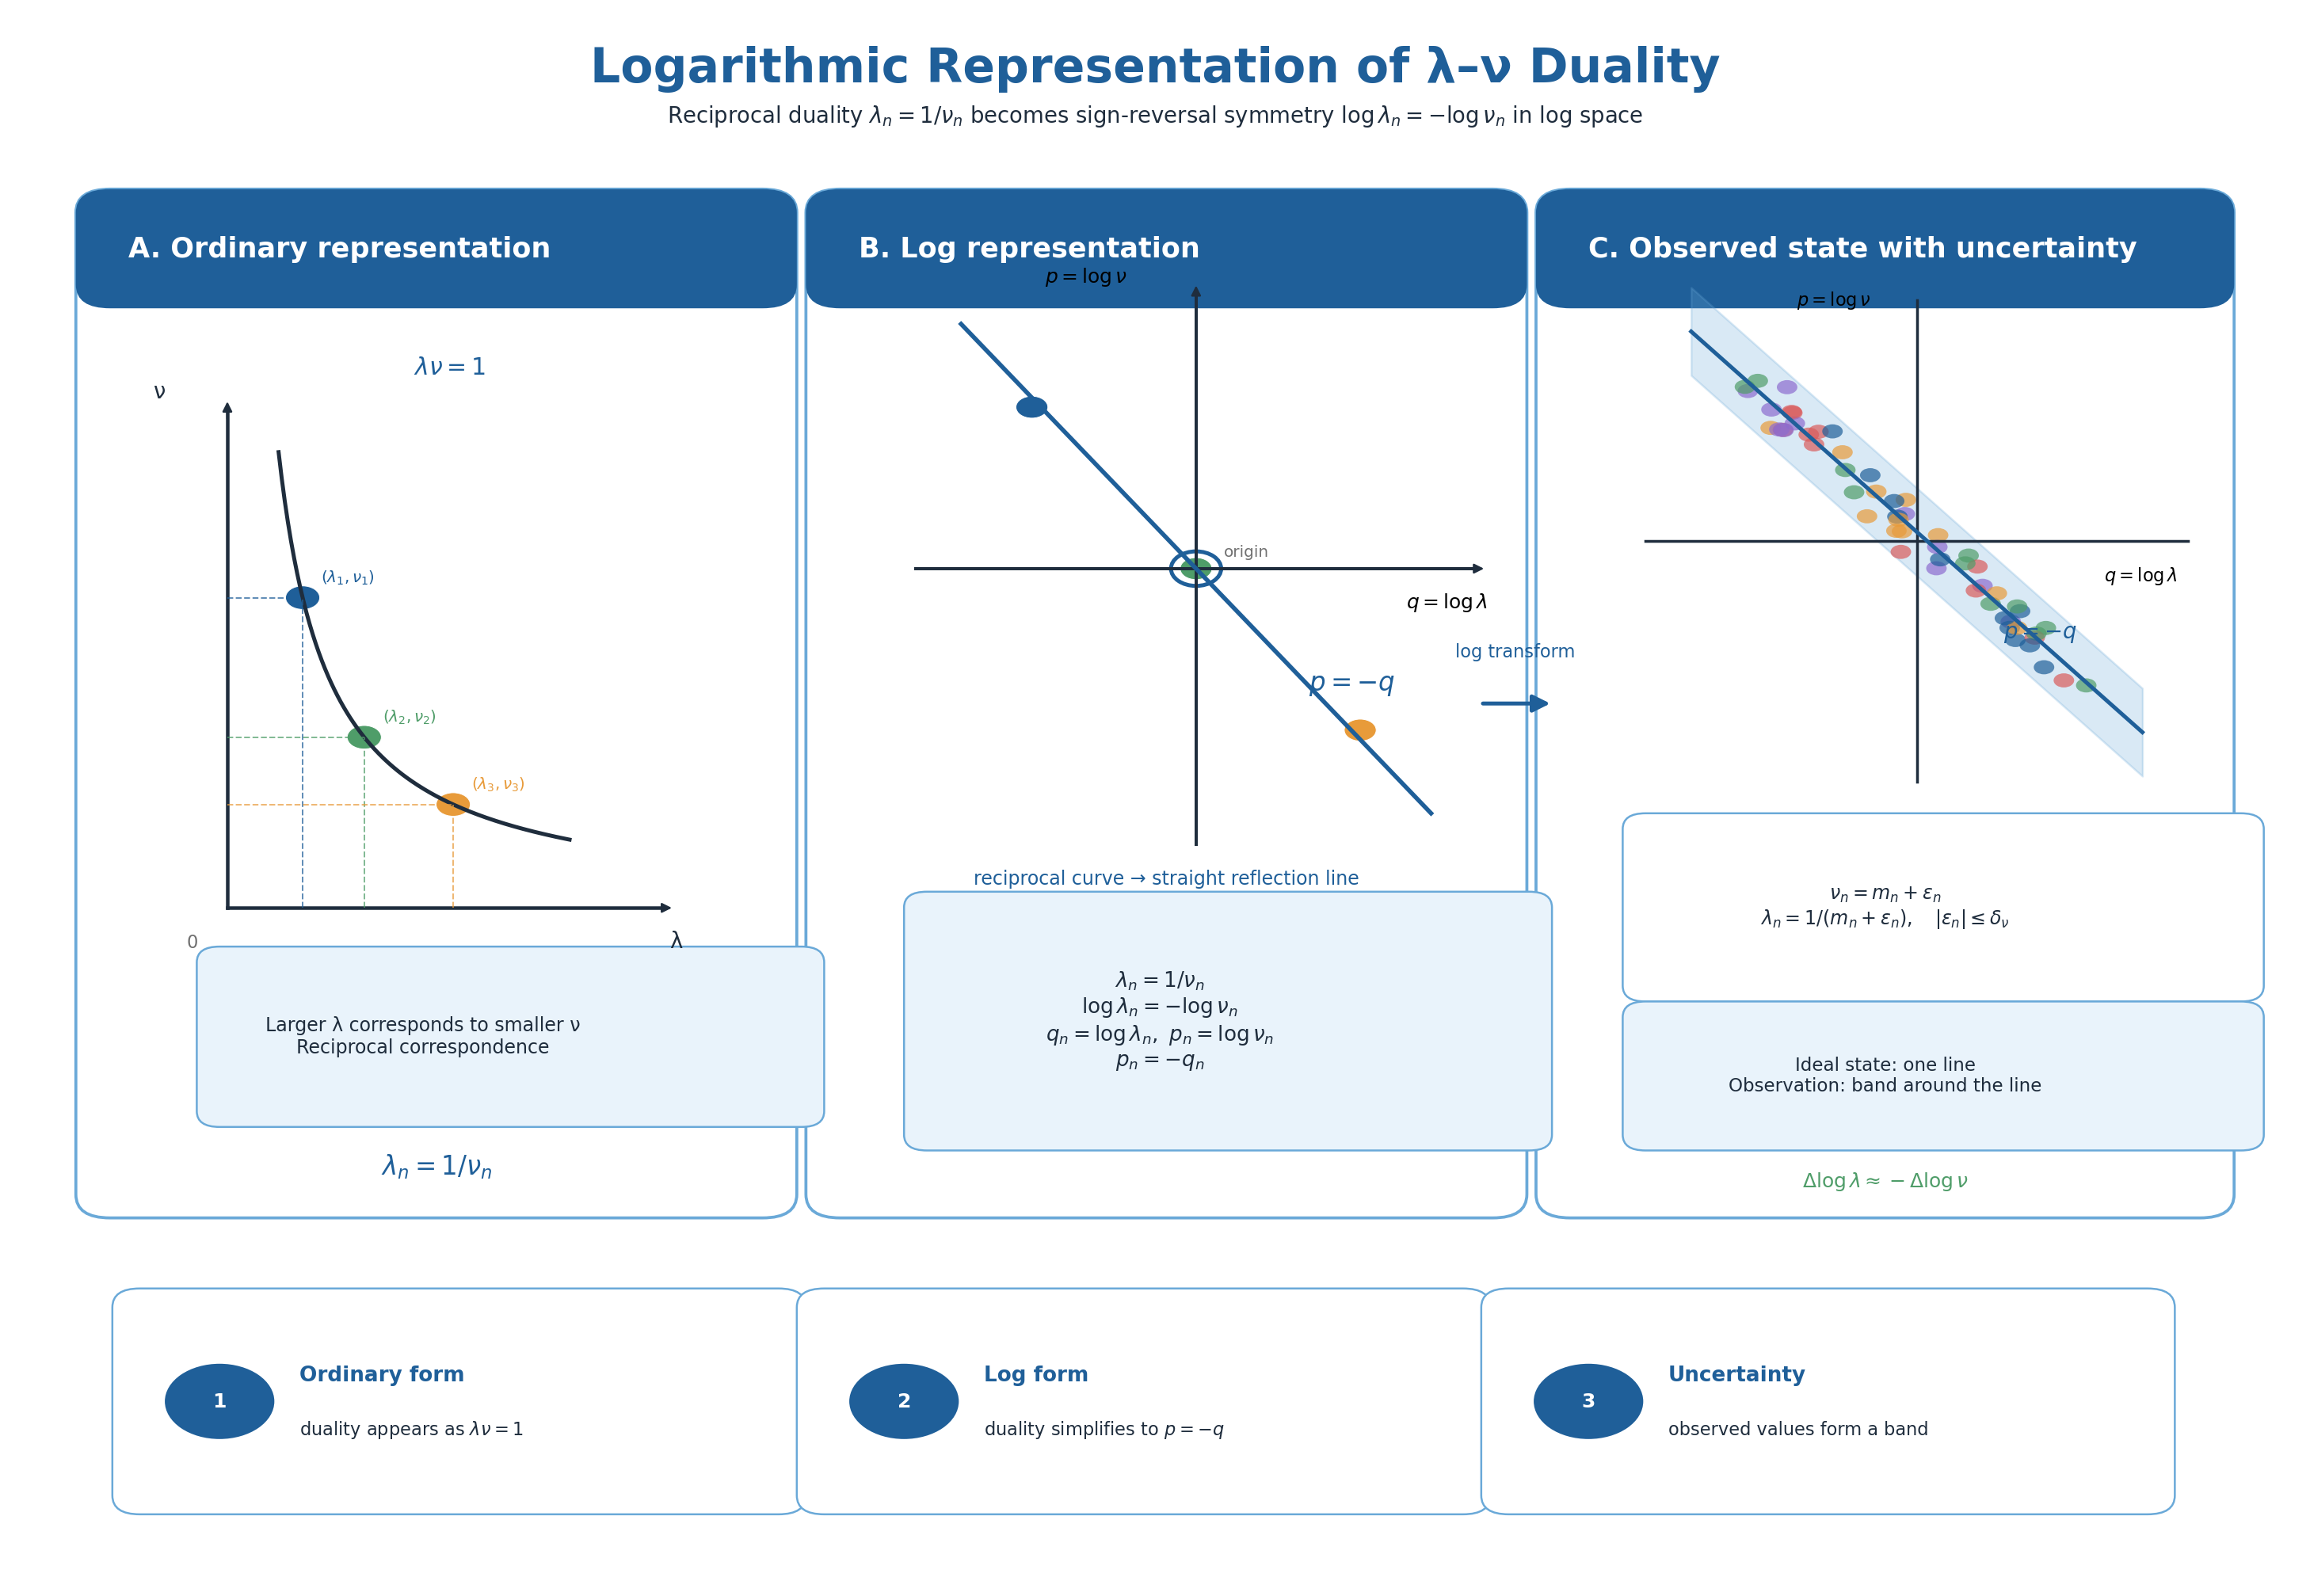
\includegraphics[keepaspectratio,alt={Logarithmic representation of the \textbackslash lambda--\textbackslash nu duality}]{./figure2_log_representation_lambda_nu_duality_EN.png}}
\caption{Logarithmic representation of the \(\lambda\)--\(\nu\) duality}
\end{figure}

\textbf{Figure 2.} The reciprocal duality, which in the ordinary
representation is the hyperbola \(\lambda\nu=1\), is expressed as the
straight line \(p=-q\) by using the logarithmic variables
\(q=\log\lambda\), \(p=\log\nu\). In an observed state with uncertainty,
it can be represented as a band-like distribution with thickness around
the ideal line. However, this paper does not determine that thickness.

\begin{center}\rule{0.5\linewidth}{0.5pt}\end{center}

\subsection{8. Counting a 4-Dimensional Lattice in an Actual Frequency /
Wavelength
Space}\label{counting-a-4-dimensional-lattice-in-an-actual-frequency-wavelength-space}

The discussion so far has mainly treated continuous dual spaces.
However, if we actually choose the frequency space or the wavelength
space to be a 4-dimensional lattice, the sum-of-squares condition is
naturally converted into a unit-cell counting problem.

\subsubsection{\texorpdfstring{8.1 Fully-inscribed counting for
\(\delta=0\)}{8.1 Fully-inscribed counting for \textbackslash delta=0}}\label{fully-inscribed-counting-for-delta0}

Consider the 4-dimensional integer lattice

\[
k=(k_1,k_2,k_3,k_4)\in\mathbb{Z}^4 .
\]

Associate to each lattice point \(k\) a 4-dimensional unit cell of side
1. The half-width of the unit cell in each direction is \(1/2\).

The condition that this entire unit cell be fully inscribed in the
4-dimensional hyperball of radius \(R\) is

\[
\sum_{i=1}^{4}
\left(|k_i|+\frac12\right)^2
\le R^2 .
\]

We therefore define the fully-inscribed cell count for \(\delta=0\) as

\[
N_0(R)
=
\#\left\{
k\in\mathbb{Z}^4
\mid
\sum_{i=1}^{4}
\left(|k_i|+\frac12\right)^2
\le R^2
\right\} .
\]

This definition applies in the same form whether a 4-dimensional lattice
is chosen in the frequency space or in the wavelength space. What is
being counted here is not a particular physical quantity but the
geometric number of 4-dimensional lattice cells subject to a
sum-of-squares constraint.

Counting in order of integer radius, for example,

\[
N_0(1)=1,\qquad
N_0(2)=9,\qquad
N_0(3)=137 .
\]

In particular, the 137 obtained at \(R=3\) is not introduced under any
assumed correspondence with a physical constant. It is a pure counting
result obtained from the 4-dimensional integer lattice, the unit cell,
and the full-inscription condition.

\subsubsection{8.2 Form of counting with
uncertainty}\label{form-of-counting-with-uncertainty}

In the fully-inscribed counting without uncertainty, each cell is
counted as 1 if it satisfies the condition and 0 otherwise. This is
counting by the indicator function

\[
\mathbf{1}[x\ge 0] .
\]

Here, define

\[
D_R(k)
=
R^2-
\sum_{i=1}^{4}
\left(|k_i|+\frac12\right)^2 .
\]

If

\[
D_R(k)\ge0 ,
\]

then that unit cell is fully inscribed in the hyperball of radius \(R\).

In the case with uncertainty, the indicator function is replaced by a
weight function

\[
W_\delta(x)
\]

having thickness near the boundary.

The effective cell count is then defined as

\[
N_\delta(R)
=
\sum_{k\in\mathbb{Z}^4}
W_\delta\!\left(
D_R(k)
\right) .
\]

The weight function is assumed to satisfy at least the following
properties,

\[
0\le W_\delta(x)\le1 ,
\]

\[
\lim_{\delta\to0}
W_\delta(x)
=
\mathbf{1}[x\ge0] .
\]

Therefore,

\[
\lim_{\delta\to0}N_\delta(R)=N_0(R) .
\]

By this formulation, the fully-inscribed counting is expressed as the
\(\delta=0\) limit of the weighted counting with uncertainty.

However, this paper does not derive the explicit form of \(W_\delta\),
the value of \(\delta\), or on which geometric quantity \(\delta\)
depends. Hence this paper does not perform a concrete numerical
evaluation of \(N_\delta(R)\).

\subsubsection{8.3 Remark on dual
counting}\label{remark-on-dual-counting}

When a 4-dimensional lattice is placed in the frequency space, one can
perform a unit-cell counting corresponding to the sum-of-squares
condition

\[
\sum_{i=1}^{4} \nu_i^2\le \mathcal{N}^2 .
\]

On the other hand, when a 4-dimensional lattice is placed in the
wavelength space, one can perform a unit-cell counting corresponding to

\[
\sum_{i=1}^{4} \lambda_i^2\le \Lambda^2 .
\]

Formally these are the same counting problem. However, since the
wavelength space and the frequency space are dually connected by

\[
\lambda_i\nu_i=1 ,
\]

when both are simultaneously discretized into lattices, the lattice
structures of the two spaces do not necessarily coincide in a simple
way.

We therefore distinguish the following two in this paper.

\begin{enumerate}
\def\labelenumi{\arabic{enumi}.}
\tightlist
\item
  The counting when the frequency space or the wavelength space alone is
  chosen as a 4-dimensional lattice.\\
\item
  The consistency condition when both are simultaneously connected by
  the reciprocal duality condition.
\end{enumerate}

This paper confines itself to defining the single-space counting of (1).
Counting that includes the dual consistency condition of (2) is left to
subsequent work.

\begin{center}\rule{0.5\linewidth}{0.5pt}\end{center}

\subsection{9. Related Work and
Positioning}\label{related-work-and-positioning}

This paper is not a modification of an existing physical theory; it is a
model that observes the geometric structure arising when a reciprocal
duality condition is placed between the wavelength space and the
frequency space. Accordingly, the following related work is referred to
not as physical grounds for the claims of this paper but as mathematical
background.

First, the idea of treating the time domain and the frequency domain
complementarily in signal analysis has a classical background
represented by Gabor's time--frequency analysis. Gabor presented a
method of treating time and frequency symmetrically in the analysis of
communication signals {[}1{]}. This paper does not physically introduce
a time axis, but it shares the formal motivation of placing dual spaces
side by side and observing them.

Second, regarding the abstraction of the frequency domain and of
information representation, Shannon's theory of communication provides a
classical background {[}2{]}. However, this paper does not treat
information content or channel capacity.

Third, the 4-dimensional lattice cell counting at the end of this paper
belongs to the context of the geometry of numbers, which treats lattice
points or lattice cells inside convex bodies. In particular, the
geometry of numbers since Minkowski has systematically treated the
relations among convex bodies, lattices, volumes, and counting {[}3{]}.

Fourth, the sum-of-squares condition on the 4-dimensional lattice is
formally close to the representation number of a sum of four squares.
However, what this paper treats is an inequality condition based on sums
of positive odd squares, and it does not directly apply Jacobi's
four-square theorem {[}4{]}.

\begin{center}\rule{0.5\linewidth}{0.5pt}\end{center}

\subsection{10. Limitations and Future
Work}\label{limitations-and-future-work}

This paper has clear limitations.

First, this paper does not complete a physical theory. Although it uses
terms such as wavelength, frequency, norm preservation, and uncertainty,
it does not directly identify them with existing physical quantities.

Second, the physical dimensions, system of units, and correspondence
with observable quantities of \(\lambda_n\) and \(\nu_n\) are undefined.

Third, we have not shown that the four-degrees-of-freedom structure is
unique. What we have shown is the observation that in one dimension the
degrees of freedom are insufficient, and that in a 5-component /
1-constraint system four degrees of freedom arise naturally.

Fourth, this paper does not determine the value or distribution of the
uncertainty width \(\delta\). In particular, the form of the weight
function \(W_\delta\) and on which quantity \(\delta\)
depends---boundary distance, shell number, dual-consistency error in
logarithmic space, etc.---are outside the scope of this paper.

Fifth, how to perform a consistent counting that simultaneously
discretizes the frequency space and the wavelength space into lattices
and further satisfies the reciprocal duality condition is left to future
work.

\begin{center}\rule{0.5\linewidth}{0.5pt}\end{center}

\subsection{11. Conclusion}\label{conclusion}

In this paper we placed the reciprocal duality condition

\[
\lambda_n=\frac{1}{\nu_n}
\]

between the wavelength components \(\lambda_n\) and the frequency
components \(\nu_n\), and observed the geometric structure that arises
when, in addition, a constant sum-of-squares condition is imposed on the
wavelength space and the frequency space respectively.

In one dimension the solution is fixed to essentially a single point,
with almost no room for redistribution among components. In contrast, a
5-component / 1-constraint system retains four degrees of freedom.

Moreover, introducing logarithmic variables, the reciprocal duality is
expressed as the sign-reversal symmetry

\[
p_n=-q_n .
\]

Finally, we showed that when the frequency space or the wavelength space
is actually chosen as a 4-dimensional lattice, the sum-of-squares
condition can be formulated as a unit-cell counting problem. In the case
without uncertainty (\(\delta=0\)), the fully-inscribed cell count
\(N_0(R)\) is obtained. Furthermore, in the case with uncertainty, it
can be formulated as the effective cell count \(N_\delta(R)\) obtained
by replacing the indicator function with a weight function \(W_\delta\).

However, this paper does not derive the value of \(\delta\) or the
explicit form of \(W_\delta\). These are outside the scope of this paper
and are left to subsequent work.

\begin{center}\rule{0.5\linewidth}{0.5pt}\end{center}

\subsection{\texorpdfstring{Appendix A: Existence Condition for the
General \(d\)-Component
System}{Appendix A: Existence Condition for the General d-Component System}}\label{appendix-a-existence-condition-for-the-general-d-component-system}

For the general \(d\)-component system, impose

\[
\sum_{n=1}^{d} \lambda_n^2=\Lambda^2,\qquad
\sum_{n=1}^{d} \nu_n^2=\mathcal{N}^2,\qquad
\lambda_n\nu_n=1 .
\]

Setting

\[
a_n=\lambda_n^2>0 ,
\]

we have

\[
\sum_{n=1}^{d} a_n=\Lambda^2,\qquad
\sum_{n=1}^{d} \frac{1}{a_n}=\mathcal{N}^2 .
\]

By a Cauchy--Schwarz type inequality,

\[
\left(\sum_{n=1}^{d} a_n\right)
\left(\sum_{n=1}^{d} \frac{1}{a_n}\right)\ge d^2 .
\]

Therefore

\[
\Lambda\mathcal{N}\ge d
\]

is a necessary condition.

\begin{center}\rule{0.5\linewidth}{0.5pt}\end{center}

\subsection{References}\label{references}

\begin{enumerate}
\def\labelenumi{\arabic{enumi}.}
\item
  Gabor, D. (1946). Theory of communication. \emph{Journal of the
  Institution of Electrical Engineers - Part III: Radio and
  Communication Engineering}, 93(26), 429--457.
\item
  Shannon, C. E. (1948). A mathematical theory of communication.
  \emph{Bell System Technical Journal}, 27(3), 379--423.
\item
  Aliev, I., \& Henk, M. (2023). Minkowski's successive minima in convex
  and discrete geometry. \emph{Communications in Mathematics}, 31(2),
  35--59.
\item
  Hirschhorn, M. D. (1987). A simple proof of Jacobi's four-square
  theorem. \emph{Proceedings of the American Mathematical Society},
  101(3), 436--438.
\end{enumerate}

\begin{center}\rule{0.5\linewidth}{0.5pt}\end{center}

\subsection{Figure Files}\label{figure-files}

\begin{itemize}
\tightlist
\item
  Figure 1: \texttt{figure1\_lambda\_nu\_dual\_constraint\_EN.png}
\item
  Figure 2:
  \texttt{figure2\_log\_representation\_lambda\_nu\_duality\_EN.png}
\end{itemize}

\end{document}
